\documentclass[]{article}

\usepackage{chronology}
\usepackage{float}
\usepackage{caption}
\usepackage{subcaption}
\usepackage{graphicx}
\usepackage{url}
\usepackage{amsmath}
\usepackage{amssymb}
\usepackage{amsthm}
\usepackage{tocloft}
\usepackage{cancel}
\usepackage{thmtools}
\usepackage[toc,nonumberlist,acronym]{glossaries}
\usepackage{glossaries-extra}
\newcommand\numberthis{\addtocounter{equation}{1}\tag{\theequation}}
\newtheorem{defn}{Definition}
\newtheorem{thm}{Theorem}
\newtheorem{lemma}[thm]{Lemma}
\graphicspath{{figs/}}
\widowpenalty10000
\clubpenalty10000
\setcounter{tocdepth}{2}

\makeglossaries
%opening
\title{Computational Neuroscience Notes}
\author{Simon Crase}

\begin{document}
\newacronym{gls:ML}{ML\glsadd{gls:mlm}}{\Gls{gls:mlm}}

\newacronym{gls:MAP}{MAP\glsadd{gls:mpm}}{\Gls{gls:mpm}}

\newglossaryentry{gls:mlm}{
	name={maximum likelihood},
	description={Choose estimator $s^*$ to maximize $p[r\vert s]$
		}}
\newglossaryentry{gls:mpm}{
	name={maximum a posteriori},
	description={Choose estimator $s^*$ to maximize $p[s \vert r]$
}}

\newglossaryentry{gls:rf}{
	name={Receptive Field},
	description={Specific properties of a sensory stimulus that generate a strong response from the cell}}
	
\maketitle

\begin{abstract}
My notes from Computational Neuroscience course
\end{abstract}

\tableofcontents
\listoffigures
\section{Introduction and Basic Neurobiology}

\subsection{Course Introduction}
\begin{figure}[H]
	\caption{Our Universes}
	\begin{subfigure}[t]{0.45\textwidth}
		\caption{According to Physicists}
		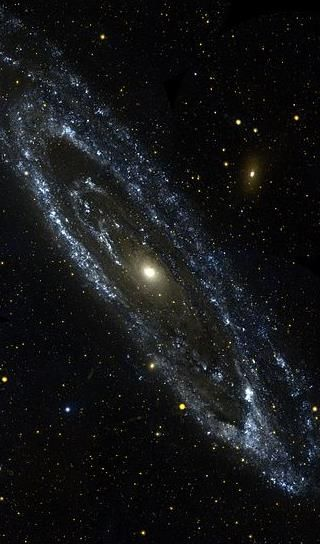
\includegraphics[width=\textwidth]{universe1}
	\end{subfigure}
	\begin{subfigure}[t]{0.45\textwidth}
		\caption{According to us}
		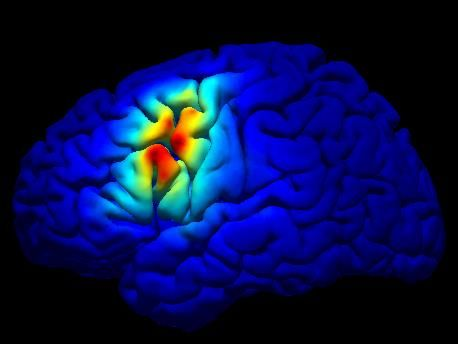
\includegraphics[width=\textwidth]{universe2}
	\end{subfigure}
\end{figure}
\subsubsection{Understanding the Brain using Computational Models}
\begin{itemize}
	\item Descriptive Models of the Brain
	\begin{itemize}
		\item How do neurons respond to external stimuli and how do we
		describe this quantitatively with a neural encoding model?
		\item How can we extract information from neurons (decoding)?
	\end{itemize}
    \item Mechanistic Models of Brain Cells and Networks
	\begin{itemize}
		\item     How can we simulate the behavior of a single neuron on a
	    computer?
	    \item How do we simulate a network of neurons?
	\end{itemize}
	\item  Interpretive (or Normative) Models of the Brain
	\begin{itemize}
		\item 	Why do brain circuits operate the way they do?
		\item What are the computational principles underlying their
		operation?
	\end{itemize}
\end{itemize}

\subsubsection{Course Goals: What you can expect to learn}
At the end of the course, you will be able to:
\begin{itemize}
	\item  Quantitatively describe what a biological neuron or
network of neurons is doing given experimental data
 \item Simulate on a computer the behavior of neurons and
networks
 \item Formulate computational principles underlying the
operation of neurons and networks in the brain
\end{itemize}

\subsection{Computational Neuroscience - Descriptive Models}


\begin{figure}[H]
	\caption{Cortical Receptive Fields}
	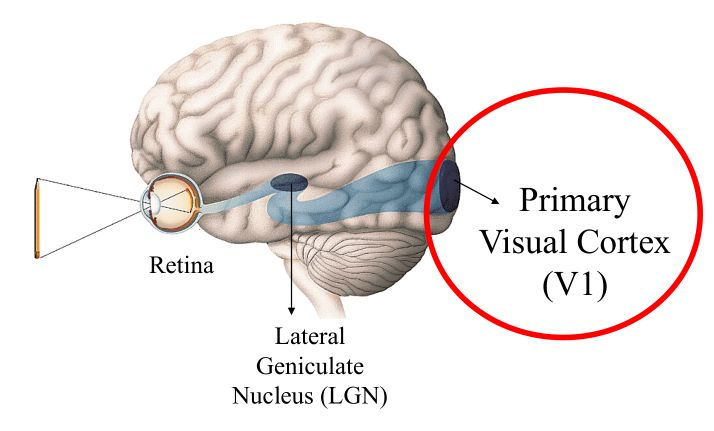
\includegraphics[width=\textwidth]{CorticalReceptive Fields}
\end{figure}

\subsection{Computational Neuroscience Mechanistic and Interpretive Models}

\subsection{The Electrical Personality of Neurons}

\subsection{Making Connections - Synapses}

\subsection{Time to Network - Brain Areas and their Function}

\begin{figure}[H]
	\caption{Brain Regions}
	\begin{subfigure}[b]{0.45\textwidth}
		\caption{Hind Brain. \emph{Medulla Oblongata} controls breathing, muscle tone and blood pressure.
			\emph{Pons} connected to the cerebellum \& involved in sleep and arousal.
			\emph{Cerebellum} Coordination and timing of voluntary movements, sense of equilibrium, language, attention}
		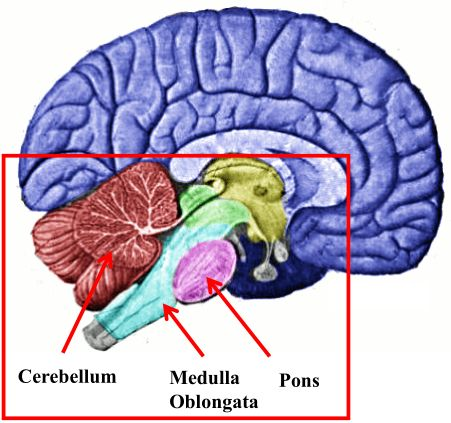
\includegraphics[width=\textwidth]{hindbrain}
	\end{subfigure}
	\begin{subfigure}[b]{0.45\textwidth}
		\caption{\emph{Midbrain} Eye movements, visual and auditory reflexes.
			\emph{Reticular Formation} 	Modulates muscle reflexes, breathing \& pain perception. Also regulates sleep, 			wakefulness \& 	arousal.}
		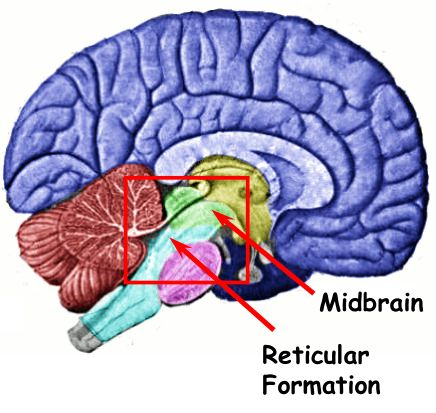
\includegraphics[width=\textwidth]{midbrain}
	\end{subfigure}
	\begin{subfigure}[b]{0.45\textwidth}
		\caption{\emph{Thalamus} Relay station for all 	sensory info (except 	smell) to the cortex, regulates sleep/wakefulness.
		\emph{Hypothalamus} Regulates basic needs: 	Fighting, Fleeing, 	Feeding, and Mating.}
		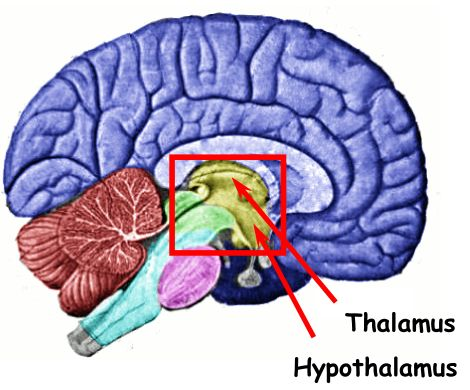
\includegraphics[width=\textwidth]{thalamus}
	\end{subfigure}
	\begin{subfigure}[b]{0.45\textwidth}
		\caption{ Consists of: Cerebral cortex, basal ganglia, 			hippocampus, and amygdala
		Involved in perception 	and motor control, 	cognitive functions,	emotion, memory, and learning}
		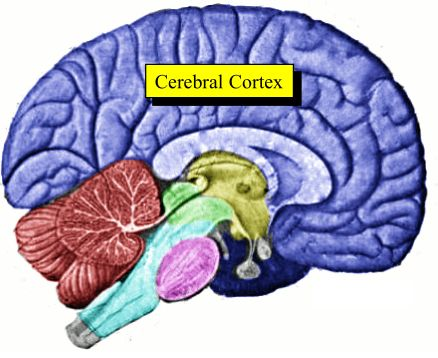
\includegraphics[width=\textwidth]{Cerebrum}
	\end{subfigure}
\end{figure}
\section{What do Neurons Encode?}
\subsection{What is the Neural Code}
\subsection{Neural Encoding - Simple Models}
\subsection{Neural Encoding - Feature Selection}
\subsection{Neural Encoding - Variability}
\section{Extracting Information from Neurons}

\subsection{Neural Decoding and Signal Detection Theory}

\begin{figure}[H]
		\caption[Value of threshold that maximizes probability of correct call]{This value of threshold maximizes probability of calling correctly.
			$p[+]p[r\ge z\vert +] + p[-] (1-p[r\ge z\vert -])$}
		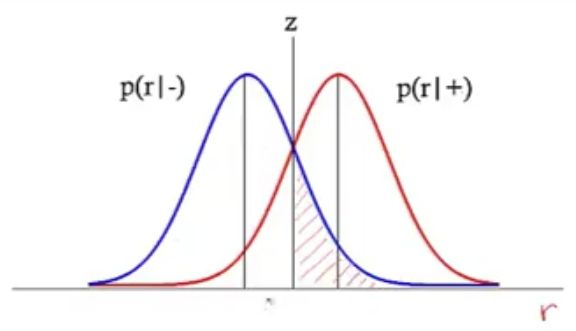
\includegraphics[width=\textwidth]{signal-detection1}
\end{figure}
\subsection{Population Coding and Bayesian Estimating}

\begin{align*}
	\underbrace{p[s\vert r]}_\text{A posteriori distribution} =& \frac{\overbrace{p[r\vert s]}^\text{Likelihood function} \cdot \overbrace{p[s]}^\text{Prior distribution}}{\underbrace{p[r]}_\text{Marginal distribution}} \text{, where}\\
	p[r] =& \int ds \; p[r\vert s] p[s]
\end{align*}

\begin{itemize}
	\item \gls{gls:ML} \gls{gls:mlm}
	\item \gls{gls:MAP} \gls{gls:mpm}
\end{itemize}
 An example. Assume:
 
\begin{enumerate}
	\item a population of neurons that encode some stimulus $s$
	\item response is Gaussian (e.g. V1)
	\item each fires independently
	\item Poisson Firing\label{item:poisson}
\end{enumerate}

\begin{figure}[H]
	\caption{Gaussian Tuning Curves}
	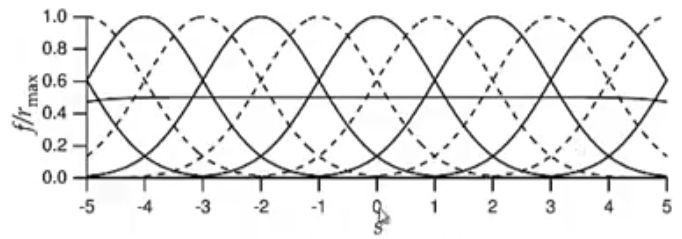
\includegraphics[width=\textwidth]{decode-stimulus}
\end{figure}

\begin{align*}
	f_a(s) =& r_{max} \exp \Big(-\frac{1}{2}\big[\frac{s-s_a}{\sigma_a}\big]^2\Big)\text{, assume good coverage} \numberthis \label{eq:gauss}\\
	\sum_{1}^{N} f_a(s) =& const \numberthis \label{eq:good:coverage}
\end{align*}

So firing rate doesn't depend on stimulus

From assumption \ref{item:poisson}, spikes are produced randomly and independently in each time bin with probability
\begin{align*}
	P_T[k] =& \frac{(rT)^k \exp (-rT)}{k!}\\
	P_T[r_a\vert s] =& \frac{(f_a(s)T)^{r_aT} \exp (-f_a(s)T)}{r_aT!}\\
	P[\vec{r}\vert s] =& \prod_{a=1}^{N}P_r[a\vert s]\\
	=& \prod_{a=1}^{N} \frac{(f_a(s)T)^{r_aT} \exp (-f_a(s)T)}{r_aT!}
\end{align*}

We want the \gls{gls:ML} for $s$.
\begin{align*}
	\ln P[\vec{r}\vert s] =& \sum_{a=1}^{N} \big[r_aT \ln (f_a(s)T) -f_a(s)T - \ln (r_aT!) \big] \text{, so we need}\\
	\nabla_a \ln P[\vec{r}\vert s] =& 0	
\end{align*}
 where  $\nabla_a$ denotes the operator $\frac{\partial}{\partial_{s_a}}$. Now
\begin{align*}
	\nabla_a \ln P[\vec{r}\vert s] = & \partial_a \sum_{a=1}^{N}  r_aT \ln (f_a(s)T) -\underbrace{\partial_a \sum_{a=1}^{N} f_a(s)T}_{=0 \text { from ]\eqref{eq:good:coverage}}} - \underbrace{\partial_a \sum_{a=1}^{N} \ln (r_aT!)}_{=0} 
\end{align*}
Hence the \gls{gls:mlm} is given by:
\begin{align*}
	T \partial_a \sum_{a=1}^{N} r_a  \ln (f_a(s)T) =& 0\\
	 \sum_{a=1}^{N} r_a  \partial_a \ln (f_a(s)T) =& 0\\
	 \sum_{a=1}^{N} r_a  \frac{\partial_a  (f_a(s)\cancel{T})}{(f_a(s)\cancel{T})} =& 0\\
	 \sum_{a=1}^{N} r_a  \frac{\partial_a  f_a(s^*)}{f_a(s^*)} =& 0 \numberthis \label{eq:ml:example}
\end{align*}

\begin{align*}
	\partial_a  f_a(s) =& \partial_a r_{max} \exp \Big(-\frac{1}{2}\big[\frac{s-s_a}{\sigma_a}\big]^2\Big)\\
	=&r_{max}\big[-\frac{1}{\cancel{2}} \frac{\cancel{2}(s-s_a)}{\sigma_a^2}\big] \exp \Big(-\frac{1}{2}\big[\frac{s-s_a}{\sigma_a}\big]^2\Big)\\
	=& \frac{\cancel{2}(s-s_a)}{\sigma_a^2} f_a(s) \text{, so \eqref{eq:ml:example} becomes}
\end{align*}
\begin{align*}
	\sum_{a=1}^{N} r_a  \frac{(s^*-s_a)}{\sigma_a^2} =& 0\\
	s^*  =& \frac{\sum_{a=1}^{N}   \frac{s_a r_a}{\sigma_a^2}}{\sum_{a=1}^{N} \frac{ r_a }{\sigma_a^2}}	\\
	=& \frac{\sum_{a=1}^{N}   p_a s_a r_a}{\sum_{a=1}^{N} p_a r_a} \text{, where the precision $p_a=\sigma_a^{-2}$}\\
	=& \frac{\sum_{a=1}^{N}   s_a r_a}{\sum_{a=1}^{N} r_a} \text{, if all the $s_a$ are equal}
\end{align*}

For the \gls{gls:MAP} estimate, Bayes rule gives:
\begin{align*}
	\ln p[s|r] =& \ln p[r|s] + \ln p[s] - \ln p[r]\\
	=& T \sum_{a=1}^{N}r_a \ln f_a(s) + \ln p[s] + C \text{, where $C$ does not depend on $s_a$}
\end{align*}

So the \gls{gls:MAP} estimator satisfies:
\begin{align*}
	\sum_{a=1}^{N} r_a \frac{f^\prime(a^*)}{f(a^*)} + \frac{p^\prime(s)}{p(s)}=&0\\
	s^*  =& \frac{\sum_{a=1}^{N}   \frac{s_a r_a}{\sigma_a^2}+\frac{s_{prior}}{\sigma_{prior}^2}}{\sum_{a=1}^{N} \frac{ r_a }{\sigma_a^2}+\frac{1}{\sigma_{prior}^2}}
\end{align*}
\subsection{Reading Minds - Stimulus Reconstruction}
We want an estimator, $S_{Bayes}$ that gives the "best" estimate of $s$ given $r$.

\section{Entropy \& Spike Trains}

\subsection{Information \& Entropy}

Entropy measures surprise.
\begin{align*}
	H =& - \sum_{i} p_i \log_2 p_i
\end{align*}

\begin{figure}[H]
	\begin{center}
		\caption{How about the stimulus?}
		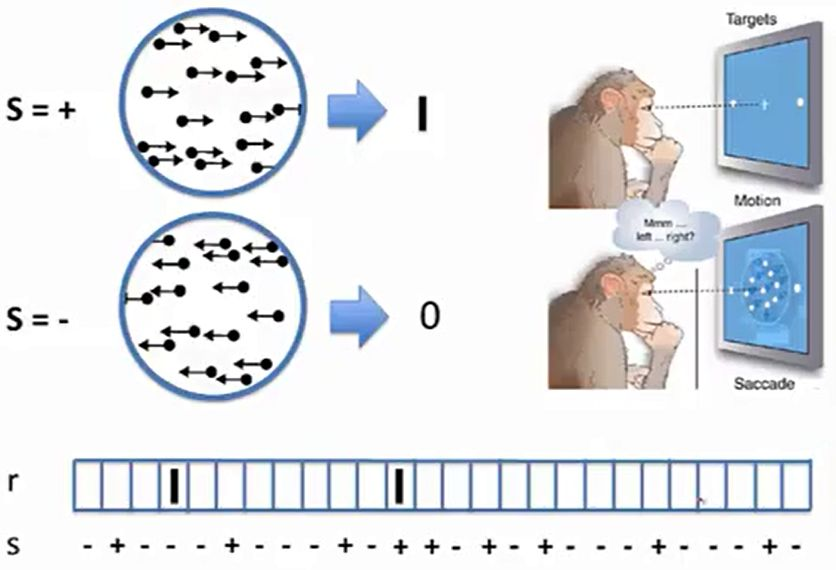
\includegraphics[width=0.8\textwidth]{how}\label{fig:how:about:the:stimulus}
	\end{center}
\end{figure}

In Figure \ref{fig:how:about:the:stimulus}, suppose the probability of error is a constant.
\begin{align*}
	P[r_-\vert +] =& q\\
	P[r_+\vert +] =& 1-q\\
	P[r_+\vert -] =& q\\
	P[r_-\vert -] =& 1-q
\end{align*}
\begin{align*}
	H[R] =& -P[r_+] \log P[r_+] - P[r_-] \log P[r_-] \text{, total entropy}\\
	H[R\vert +] =& -q \log q - (1-q) \log (1-q) \text{, noise entropy}
\end{align*}


Mutual Information: total entropy - average noise entropy.

\begin{align*}
	I(R,S) =& -\sum_r p[r] \log p[r] - \sum_s p(s)\big[- \sum_r p[r \vert s] \log p[r \vert s]\big]\\
	=& H[R] - \sum_s p(s) H[R\vert s]\\
\end{align*}
\begin{align*}
	I[S,R] \triangleq D_{KL}&\big[P(R,S),P(R)P(S)\big]\\
	=&H[R]-\sum_s P(s) H[R\vert s]
\end{align*}

\subsection{Calculating Information in Spike Trains}

\begin{figure}[H]
	\caption[Calculating Information in Spike Patterns]{Calculating Information in Spike Patterns. Divide into words of length $T$, e.g. $w_1=[1,0,1,0,1,1,0]$. Information is difference between total variability driven by stimuli and that dues to noise, averaged over stimuli.}
	\includegraphics*[width=\textwidth]{calculatingInformationInSpikePatterns}
\end{figure}


\appendix

\printglossaries

\end{document}
